%%%%%%%%%%%%%%%%%%%%%%%%%%%%%%%%%%%%%%%%%%%%%%%%%%
% FORMATING UNTUK BUKU
%%%%%%%%%%%%%%%%%%%%%%%%%%%%%%%%%%%%%%%%%%%%%%%%%%
\documentclass[a5paper,11pt,twoside]{book}
\usepackage{blindtext}
\usepackage{geometry}
\usepackage{titlesec}
\usepackage{hyperref}
\usepackage{afterpage}
\usepackage{indentfirst}
\usepackage{etoolbox}
\usepackage{lmodern}
\usepackage{graphicx}
\usepackage{sectsty}
\usepackage{tikz}

\graphicspath{ {./images} }

\font\tfont=cmr12 at 14pt
\sectionfont{\fontsize{12}{15}\selectfont}

\setlength{\parindent}{2em}
\setlength{\parskip}{0.5em}

%\newcommand\blankpage{%
%	\null
%	\thispagestyle{empty}%
%	\addtocounter{page}{-1}%
%	\newpage}

\hypersetup{
	colorlinks,
	citecolor=black,
	filecolor=black,
	linkcolor=black,
	urlcolor=black
}
\geometry{
	left=20mm,
	top=20mm,
	right=15mm,
	bottom=15mm,
}
\renewcommand{\chaptername}{CODE}
\renewcommand{\contentsname}{Daftar Isi}
\renewcommand{\figurename}{Gambar}
\renewcommand{\tablename}{Tabel}
\renewcommand{\listfigurename}{Daftar Gambar}
\renewcommand{\listtablename}{Daftar Tabel}

\titleformat{\chapter}[display]
{\normalfont\bfseries}
{CODE \thechapter \centering}{-2ex}
{
	\rule{\textwidth}{0pt}
	\vspace{0ex}
	\centering}
[\vspace{-5ex}\rule{\textwidth}{0pt}]

\titlespacing*{\chapter}{0pt}{-50pt}{14pt}
%%%%%%%%%%%%%%%%%%%%%%%%%%%%%%%%%%%%%%%%%%%%%%%%%%
% BEGIN BOOK
%%%%%%%%%%%%%%%%%%%%%%%%%%%%%%%%%%%%%%%%%%%%%%%%%%
\begin{document}

\title{Ensiklopedia}
\author{De Jierro}
\date{2017}

\maketitle

\chapter{PROLOG}

Sudah hampir 200 tahun setelah perang dunia ke-tiga menghancurkan 1/3 dunia. Kegilaan itu berhasil menghilangkan 60\% spesies makhluk hidup yang ada kala itu. Namun perdamaian dunia menggagalkan kelanjutan perang tersebut dan memberikan pandangan baru kepada dunia. Inofasi energi masal selain nuklir telah ditemukan kala berakhirnya kegilaan yang dahulu. Sebuah gedung riset pabrik senjata meledak dan menghancurkan 1/3 dunia. Jika perang dunia berakhir karena telah terjadi ledakan rudal(nuklir), namun kali ini karena kegagalan pembuatan rudal tipe terbaru. Kini perdamaian dunia terjalin, sisi terang dunia sudah mulai berinar bersinar lagi. Namun semakin terang cahaya yang bersinar akan semakin gelap bayangannya.

Terbangun aku dimalam hari. Dingin angin malam berhembus membuatku menggigil. Suara raungan perut kosong meramaikan kamar kecil yang hanya seukuran 2x2 tinggi manusia dewasa rata-rata. Di sisi terang dunia aku tinggal di balik bayangannya. Hanya mengenakan kaos dan celana pendek aku duduk termenung melihat langit dari jendela sembari menggam mouse PC di tangan kanan. Biarpun ku menatap langit yang hanya bisa aku lihat hanyalah awan tebal merah dengan kabut asap. Bintang bintang yang aku berasal dari tiang tiang dan tembok tembok raksasa menjulang tinggi kelangit. Ku palingkan pandangan ku ke PC tua yang sudah usang dan berdebu ini. Hampir se-abad PC tua ini digunakan turun temurun. Aku mulai merapihkan data yang sudah terkumpul tadi siang kedalam kelas dan katagori. Data yang ku kumpulkan adalah data tentang tanaman dan makhluk hidup lainnya yang masih hidup di sekitar sini dan cara untuk membudidayakannya. Ya, termasuk membudidayakan rumput dan kutu. Ku kumpulkan semua data itu setiap hari dan merangkumnya dalam sebuah database ensiklopedia yang aku terbitkan dalam artikel majalah elektronik lokal setiap minggunya. Pendapatan dari terbitan itu cukup untuk aku makan 5 hari. Tidak hanya data tentang makhluk hidup yang aku kumpulkan, semua informasi baik itu dari teknologi terbaru dan canggih hingga tetangga yang ketauan selingkuh aku kumpulkan. Namun aku tak akan mempublikasikan informasi sosial dan provokatif. Kau tau aturan negara ini, bila kau kedapatan melakukannya maka kehadiranmu akan hilang dari sejarah. Kau tahu maksudku.

\clearpage
\tikz[remember picture,overlay] \node[opacity=1.0,inner sep=0pt] at (current page.center){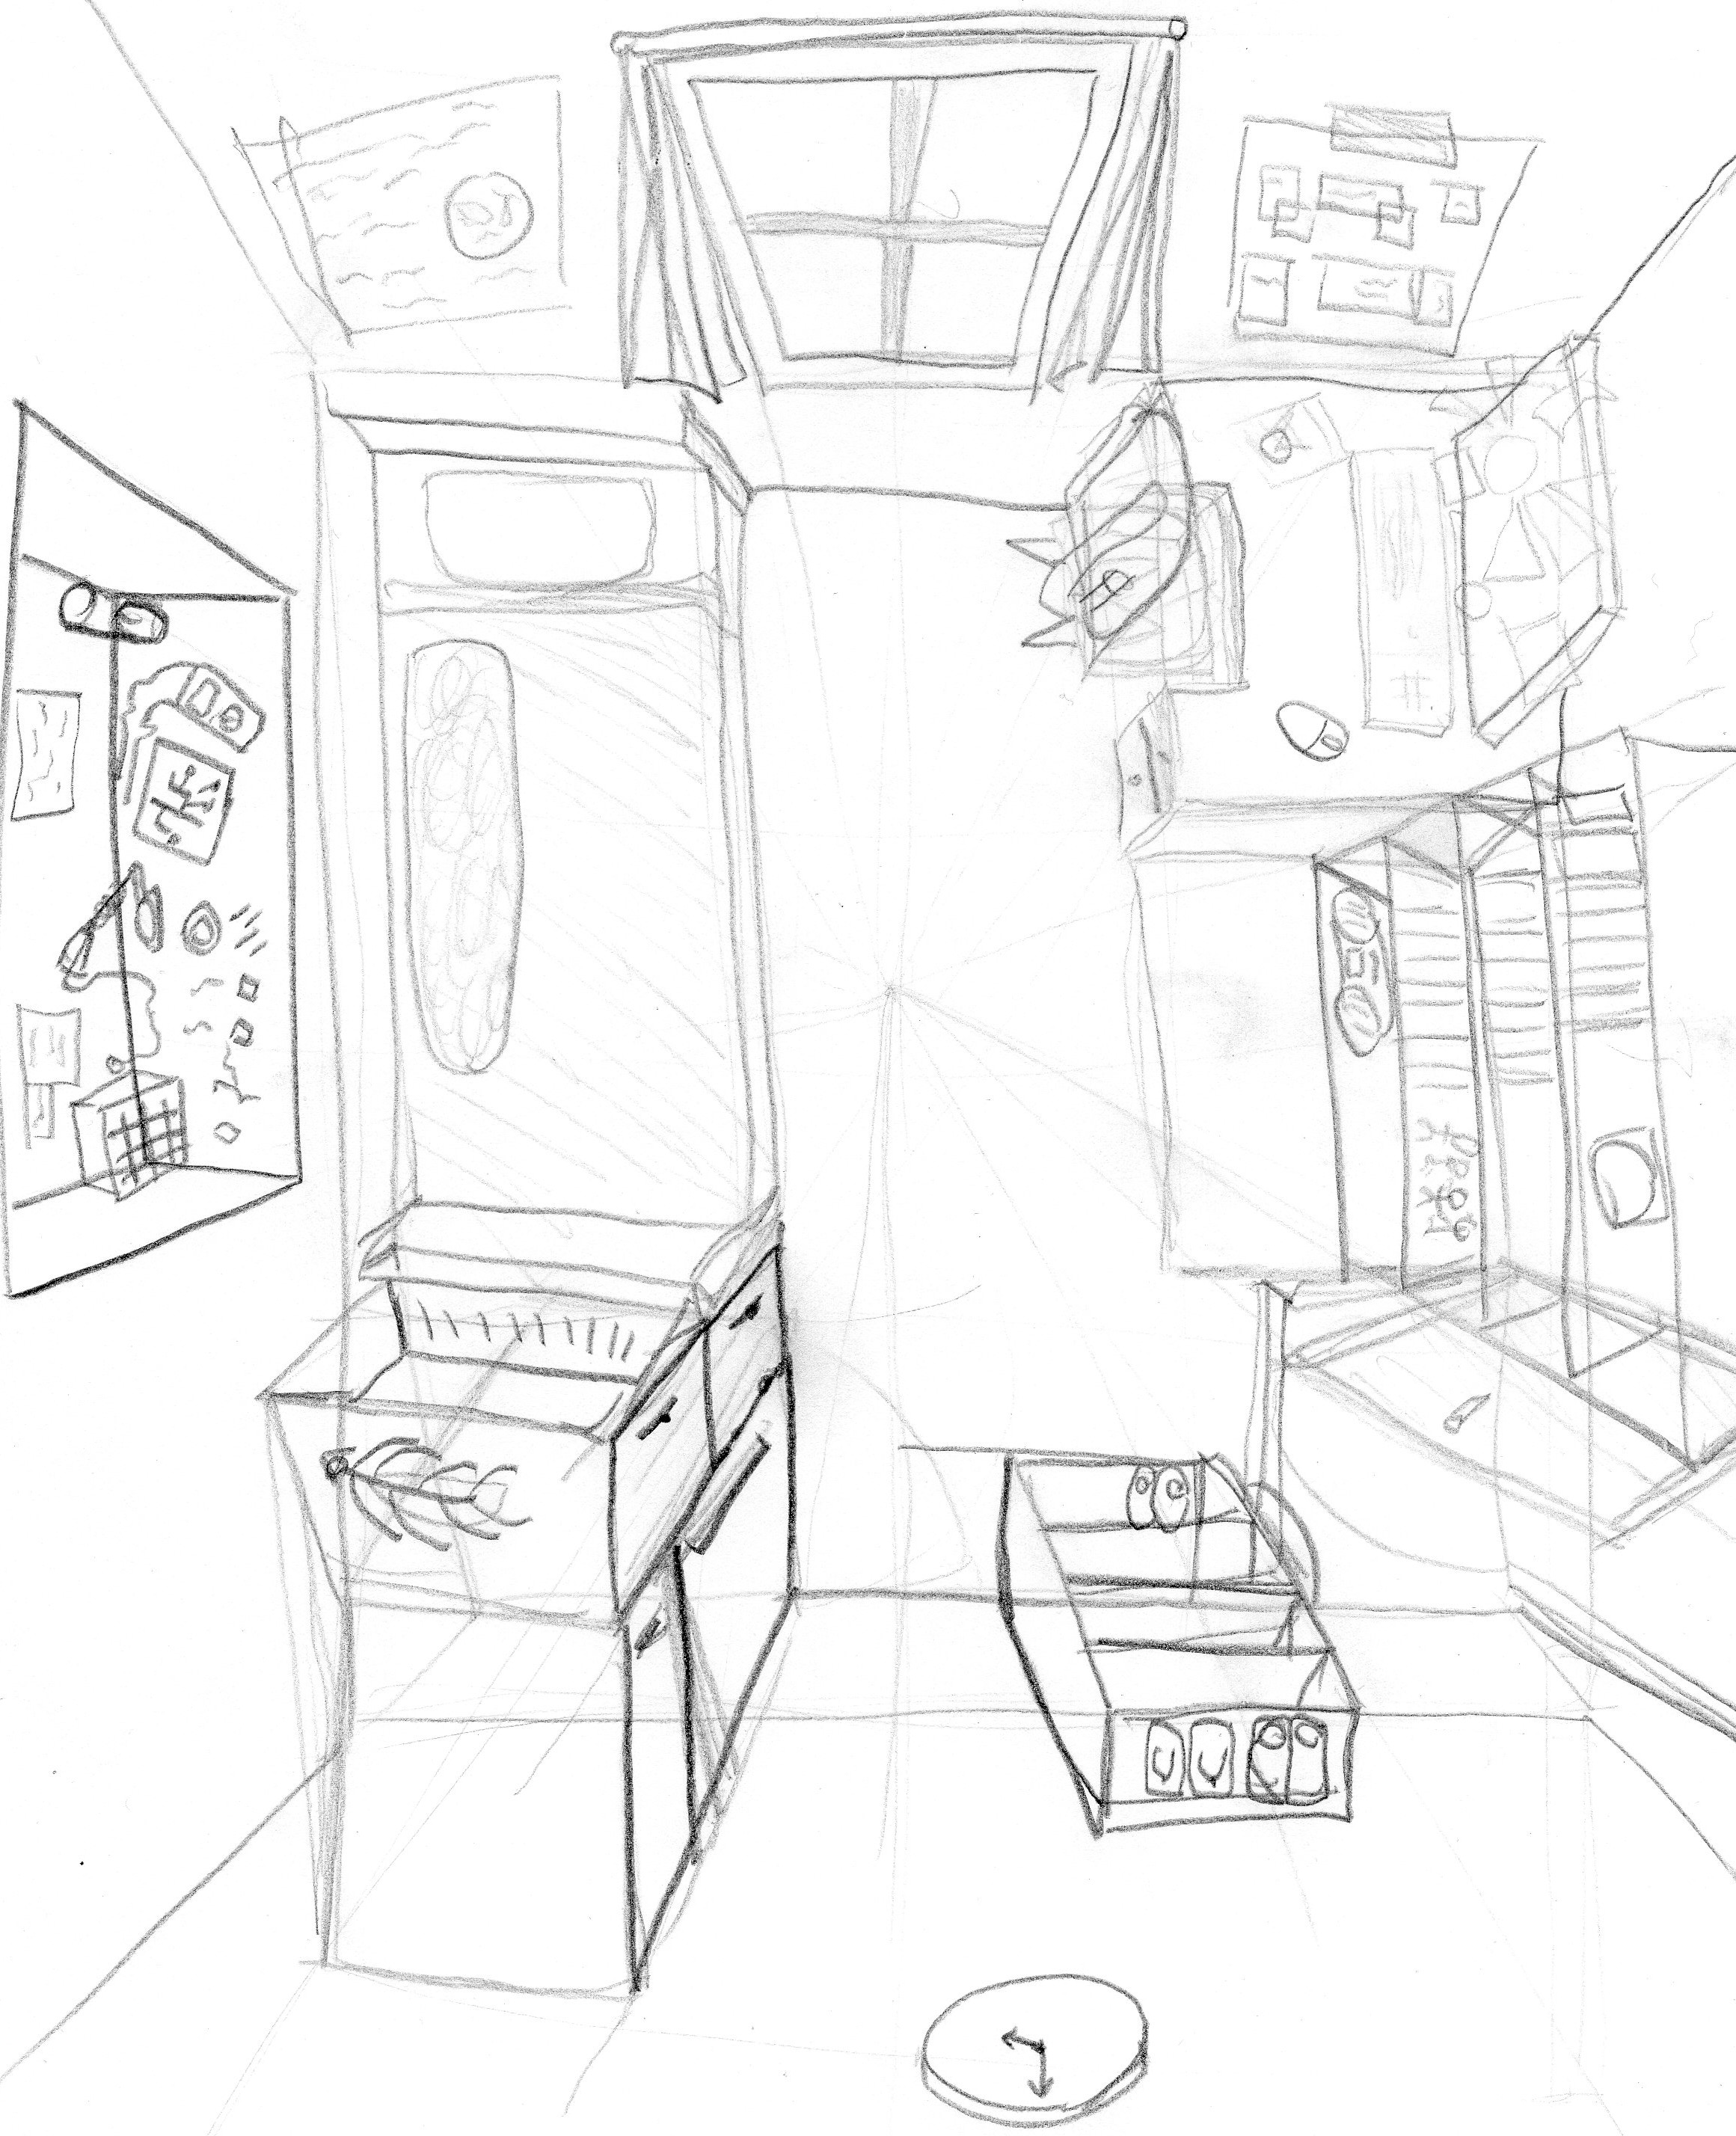
\includegraphics[width=\paperwidth,height=\paperheight]{./images/0}};
\chapter{HOBBY}

[tik tik clak tak tik clak] suara keyboard meramaikan malam ini. Barisan kode pada layar terus bertambah puluhan, ratusan, hingga ribuan baris kode terus bertambah.

[tiiiit... hngggg... sroot... srooot] dispanser cairan hitam mulai memompa cairannya, tetes demi tetes cairan hitam itu mengisi loyang selebar telapak tangan di bawah dispenser yang cukup untuk menampung 1 liter air. Beberapa saat kemudian tidak ada tetesan lagi yang menetes dan cairan hitam tersebut mulai menggumpal seperti lendir. Layaknya cairan bijih besi yang di dekatkan magnet cairan tersebut menggelembung dan mulai memadat dan tidak menampakkan bentuk seperti unsur cair sebelumnya. Di atas loyang tadi nampak sebuah sarung tangan hitam seperti yang digunakan para kesatria baju besi pada abad pertengahan.

[clang,.. sret sreat] ku ambil sarung tangan itu dan kukenakan di tangan kanan. Mengacungkan telunjuk ku seketika gumpalan lendir berkumpul di ujung telunjuk dan membentuk pisau kecil dengan 1 sisi tajam seperti cakar elang. Kemudian aku membayangkan pisau itu hilang dan pisau tadi melebur kembali membentuk gumpalan lendir dan menghilang seakan terserap ke dalam jari tangan. Aku bayangkan kembali pisau itu muncul sembari mengacungkan jari telunjuk dan setelah beberapa saat pisau tadi terbentuk. Aku goreskan pisau tadi pada meja kerja ku dan ku tulis nama ku diatas nya.

(menghela nafas) "... 10 detik kah? Aku rasa cukup untuk kali ini"

material hitam merupakan teknologi yang sudah tidak asing lagi digunakan menggantikan pasta 3d printer dan perangkat elektronik maupun mekanik bahkan pakaian sejak 25 dekade terakhir. Material ini sudah dijual bebas pada kalayak umum dalam baru pada 5 dekade lalu. Sebelumnya hanya digunakan pada keperluan militer dan juga perangkat penting negara. Namun terimakasih kepada pejabat yang korup iya menjual sebagian pabrik manufaktur material hitam kepada pengusaha asing dengan iming iming harga yang tidak bisa kau bayangkan selama 7 turunan. Akhirnya material hitam dapat dijual belikan dengan harga murah, yup semurah harga tiket pulang pergi pesawat ulak alik bumi-bulan. Namun sejak 2 tahun lalu sudah banyak perusahaan perusahaan anak cabang berdiri dan menjual meterial hitam dengan harga jauh lebih murah.

Namun proses manufakturing material hitam yang dijual bebas dengan harga yang jauh lebih murah merupakan produk gagal. Material hitam ini sering meleleh ketika digunakan dan hanya bertahan 6 bulan dengan maintanance. Dengan harga murah perusahaan sering menipu pelanggan dan menyingkat proses manufakturing tanpa melewati proses kontrol kualitas. Material hitam dengan kualitas tinggi dapat bertahan hingga bertahun tahun tanpa maintanance dan puluhan tahun dengan maintanance. Rekor menyebutkan kualitas terbaik yang pernah ada dapat bertahan selama 50 tahun.

Aku dapatkan meterial hitam dari hasil penjualan informasi di pasar gelap. Aku dapatkan dari salah seorang pekerja yang bekerja di salah satu pabrik manufakturing material hitam. Selain menulis dan menerbitkan artikel aku juga menjual informasi rahasia bagi mereka yang membutuhkan. Mungkin kau pikir seorang penulis artikel dan broker merupakan orang eksekutif VIP yang memiliki banyak kekayaan dan hidup dalam kemewahan. Tentu saja, tidak semua orang. Aku selalu habiskan uang ku untuk membeli informasi serta teknologi baru untuk ku gunakan sebagai bahan ensiklopedia pribadi ku. Yup, mengumpulkan informasi dan membukukannya dalam database ensiklopedia merupakan hobi ku. Layaknya seperti buku manual pada peralatan teknis. Kutuangkan semua informasi dan ilustrasi yang menggambarkan suatu object tertentu.

Kali ini aku sedang melakukan riset untuk mengumpulkan informasi tentang materi hitam. Dari tentang pengenalan, produksi hingga apa saja yang dapat aku lakukan dengan benda ini. Aku menikmati ini karena aku dapat berimajinasi dengan informasi yang aku miliki. Aku seorang seniman.

\clearpage
\tikz[remember picture,overlay] \node[opacity=1.0,inner sep=0pt] at (current page.center){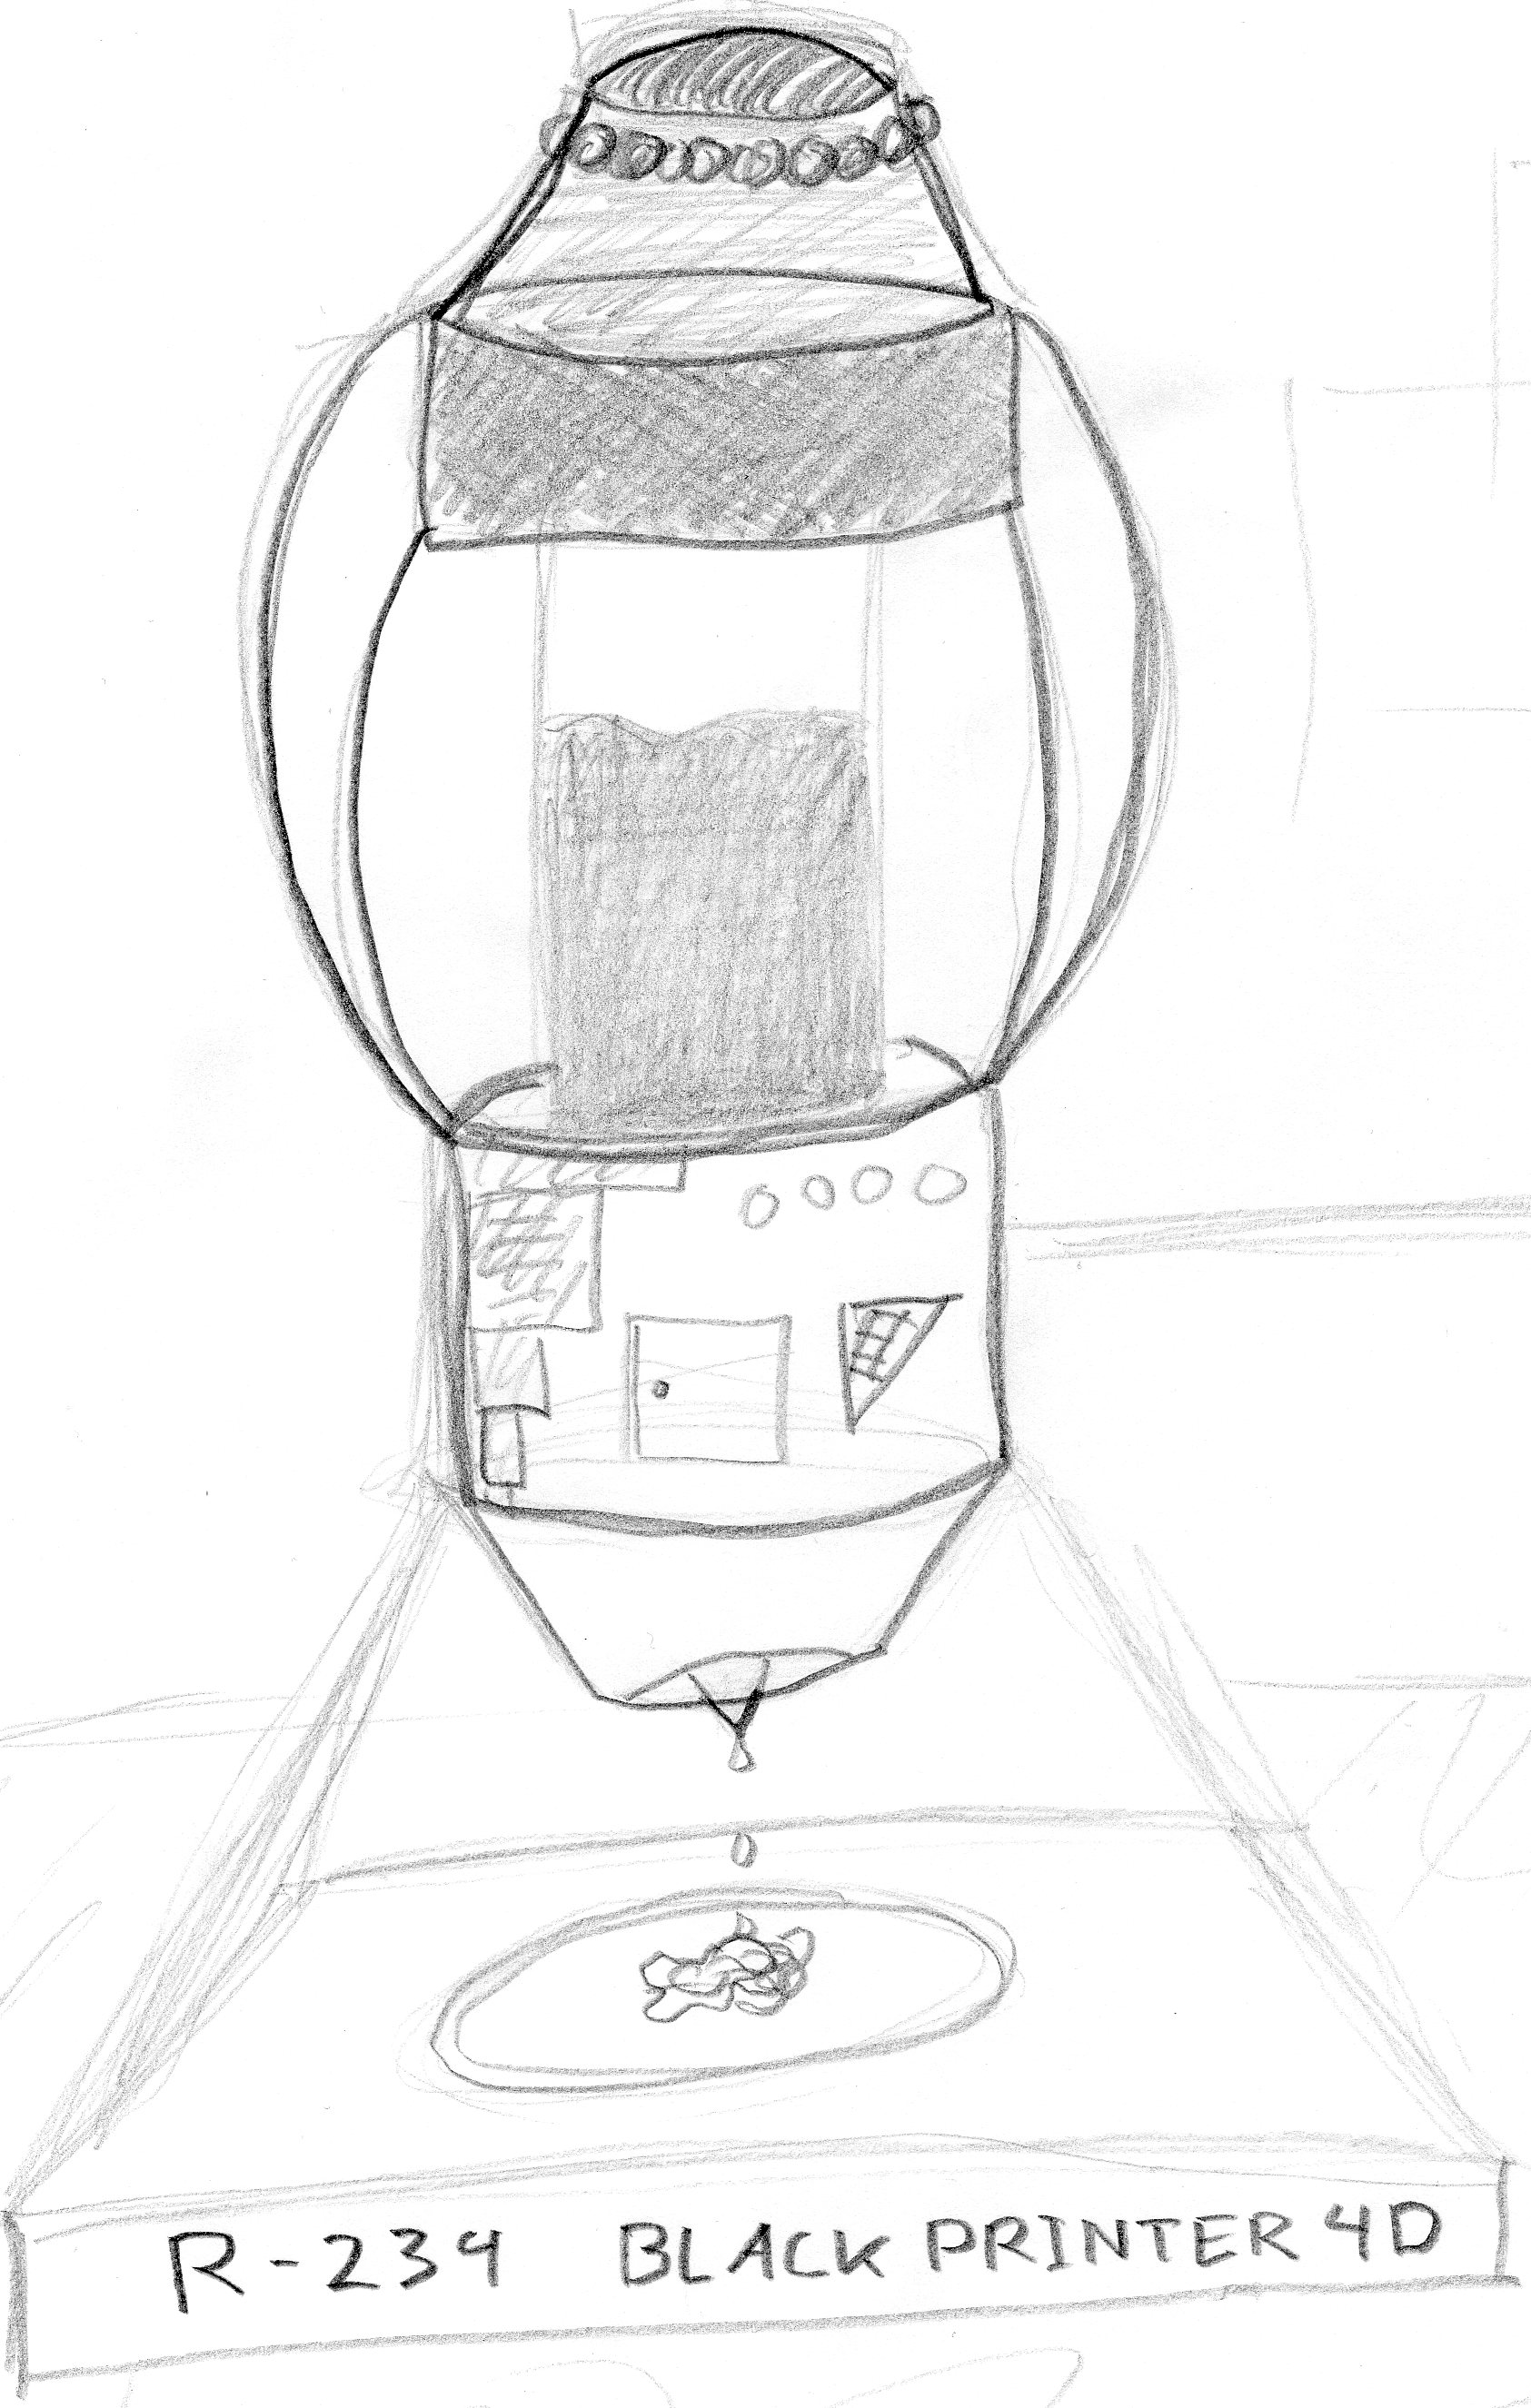
\includegraphics[width=\paperwidth,height=\paperheight]{./images/1}};
\chapter{TRADER}

[tik tik clak tak tik clak] suara keyboard meramaikan malam ini. Barisan kode pada layar terus bertambah puluhan, ratusan, hingga ribuan baris kode terus bertambah.

[tiiiit... hngggg... sroot... srooot] dispanser cairan hitam mulai memompa cairannya, tetes demi tetes cairan hitam itu mengisi loyang selebar telapak tangan di bawah dispenser yang cukup untuk menampung 1 liter air. Beberapa saat kemudian tidak ada tetesan lagi yang menetes dan cairan hitam tersebut mulai menggumpal seperti lendir. Layaknya cairan bijih besi yang di dekatkan magnet cairan tersebut menggelembung dan mulai memadat dan tidak menampakkan bentuk seperti unsur cair sebelumnya. Di atas loyang tadi nampak sebuah sarung tangan hitam seperti yang digunakan para kesatria baju besi pada abad pertengahan.

[clang,.. sret sreat] ku ambil sarung tangan itu dan kukenakan di tangan kanan. Mengacungkan telunjuk ku seketika gumpalan lendir berkumpul di ujung telunjuk dan membentuk pisau kecil dengan 1 sisi tajam seperti cakar elang. Kemudian aku membayangkan pisau itu hilang dan pisau tadi melebur kembali membentuk gumpalan lendir dan menghilang seakan terserap ke dalam jari tangan. Aku bayangkan kembali pisau itu muncul sembari mengacungkan jari telunjuk dan setelah beberapa saat pisau tadi terbentuk. Aku goreskan pisau tadi pada meja kerja ku dan ku tulis nama ku diatas nya.

(menghela nafas) "... 10 detik kah? Aku rasa cukup untuk kali ini"

material hitam merupakan teknologi yang sudah tidak asing lagi digunakan menggantikan pasta 3d printer dan perangkat elektronik maupun mekanik bahkan pakaian sejak 25 dekade terakhir. Material ini sudah dijual bebas pada kalayak umum dalam baru pada 5 dekade lalu. Sebelumnya hanya digunakan pada keperluan militer dan juga perangkat penting negara. Namun terimakasih kepada pejabat yang korup iya menjual sebagian pabrik manufaktur material hitam kepada pengusaha asing dengan iming iming harga yang tidak bisa kau bayangkan selama 7 turunan. Akhirnya material hitam dapat dijual belikan dengan harga murah, yup semurah harga tiket pulang pergi pesawat ulak alik bumi-bulan. Namun sejak 2 tahun lalu sudah banyak perusahaan perusahaan anak cabang berdiri dan menjual meterial hitam dengan harga jauh lebih murah.

Namun proses manufakturing material hitam yang dijual bebas dengan harga yang jauh lebih murah merupakan produk gagal. Material hitam ini sering meleleh ketika digunakan dan hanya bertahan 6 bulan dengan maintanance. Dengan harga murah perusahaan sering menipu pelanggan dan menyingkat proses manufakturing tanpa melewati proses kontrol kualitas. Material hitam dengan kualitas tinggi dapat bertahan hingga bertahun tahun tanpa maintanance dan puluhan tahun dengan maintanance. Rekor menyebutkan kualitas terbaik yang pernah ada dapat bertahan selama 50 tahun.

Aku dapatkan meterial hitam dari hasil penjualan informasi di pasar gelap. Aku dapatkan dari salah seorang pekerja yang bekerja di salah satu pabrik manufakturing material hitam. Selain menulis dan menerbitkan artikel aku juga menjual informasi rahasia bagi mereka yang membutuhkan. Mungkin kau pikir seorang penulis artikel dan broker merupakan orang eksekutif VIP yang memiliki banyak kekayaan dan hidup dalam kemewahan. Tentu saja, tidak semua orang. Aku selalu habiskan uang ku untuk membeli informasi serta teknologi baru untuk ku gunakan sebagai bahan ensiklopedia pribadi ku. Yup, mengumpulkan informasi dan membukukannya dalam database ensiklopedia merupakan hobi ku. Layaknya seperti buku manual pada peralatan teknis. Kutuangkan semua informasi dan ilustrasi yang menggambarkan suatu object tertentu.

Kali ini aku sedang melakukan riset untuk mengumpulkan informasi tentang materi hitam. Dari tentang pengenalan, produksi hingga apa saja yang dapat aku lakukan dengan benda ini. Aku menikmati ini karena aku dapat berimajinasi dengan informasi yang aku miliki. Aku seorang seniman.

\clearpage
\tikz[remember picture,overlay] \node[opacity=1.0,inner sep=0pt] at (current page.center){
\includegraphics[width=\paperwidth,height=\paperheight]{./images/00}};
\end{document}